\subsubsection{Artificial neural network}

\textbf{Goal \& parameters:} Like in ANN regression, the goal is to produce a mapping from $M$ input variables to $D$ output variables. But what are $M, D$ and $H$ now? We want to predict a the glass type based on the 9 continuous input variables, so $M = 9$. We want the ANN to output the \textit{probability} of the observation being the glass types \texttt{type1} through \texttt{type7}, so $D=7$. Given such a list of probabilities, we select the type corresponding to the highest probability. Like in the ANN regression, we choose the optimal $H$ based on cross-validation.

% \textbf{Algorithm:} Our algorithm for ANN classification is almost identical to our ANN regression algorithm, with two notable exceptions: The outer CV split uses stratified hold-out, and error functions now check for equality. I.e. if predicted class $\neq$ actual class, the error count is increased by 1. 

\begin{multicols}{2}
\textbf{Results:} The validation error initially decreased, then stabilized around 25 \% for $H \geq 7$, as seen in fig \ref{fig:ANN_class_validation_error}. The algorithm chose $H=7$ as the optimal number of hidden nodes. In the final test, the estimated generalization error was $\hat{E}^{\text{gen}} = 0.2857 \approx 28.6 \, \%$. Fig \ref{fig:ANN_class_decision_boundaries} shows the decision boundaries determined by the training partition, and the test observations in from the final test. Since each data points exists in a high 9-dimensional space, the plot shows the points projected onto the two principal components. As discussed in report 1, the first two principal components account for only $\approx 50 \, \%$ of the variance in the data, so this PCA projection is not a fantastic representation of the data.

\begin{figure}[H]
    \centering
    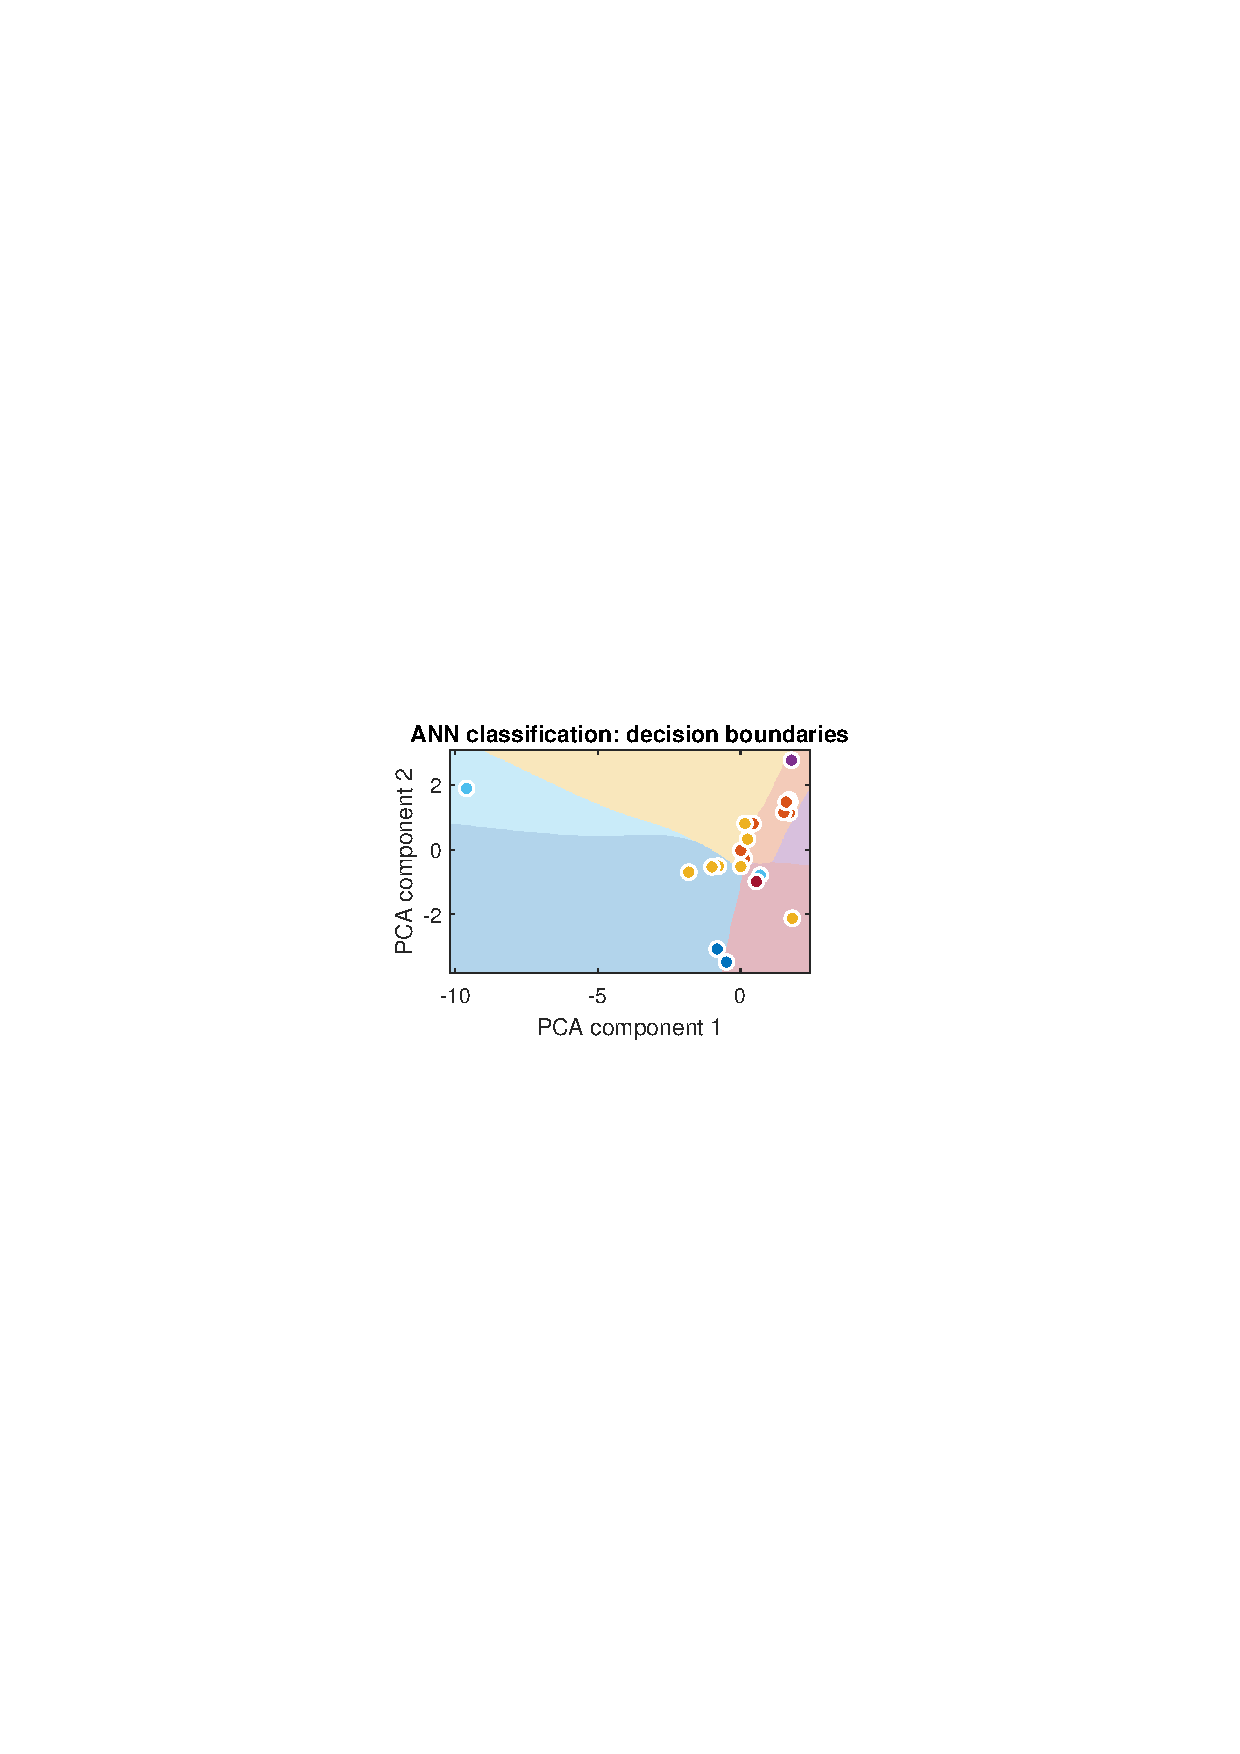
\includegraphics[width=0.50\textwidth]{fig/classification/ANN_class_decision_boundaries.pdf}
    \caption{The decision boundaries determined by the training partition, and the test observations in the final test.}
    \label{fig:ANN_class_decision_boundaries}
\end{figure}
\end{multicols}

The average probability of the predicted guess in the final test was 75 \%. As seen in fig \ref{fig:ANN_class_predicted_vs_actual}, when the ANN outputs a high probability for a prediction, it is likely correct; when it outputs a low probability, it is less likely to predict correctly, as expected. A potential improvement could be obtained by using regularization. 

\textbf{Trained network:} Since the trained network has $M = 8$ input nodes, $H=7$ hidden nodes,  and $D=7$ output nodes, the trained network is difficult to visualize. It is shown in appendix. 

\begin{multicols}{2}
\newpage
\begin{figure}[H]
\centering
    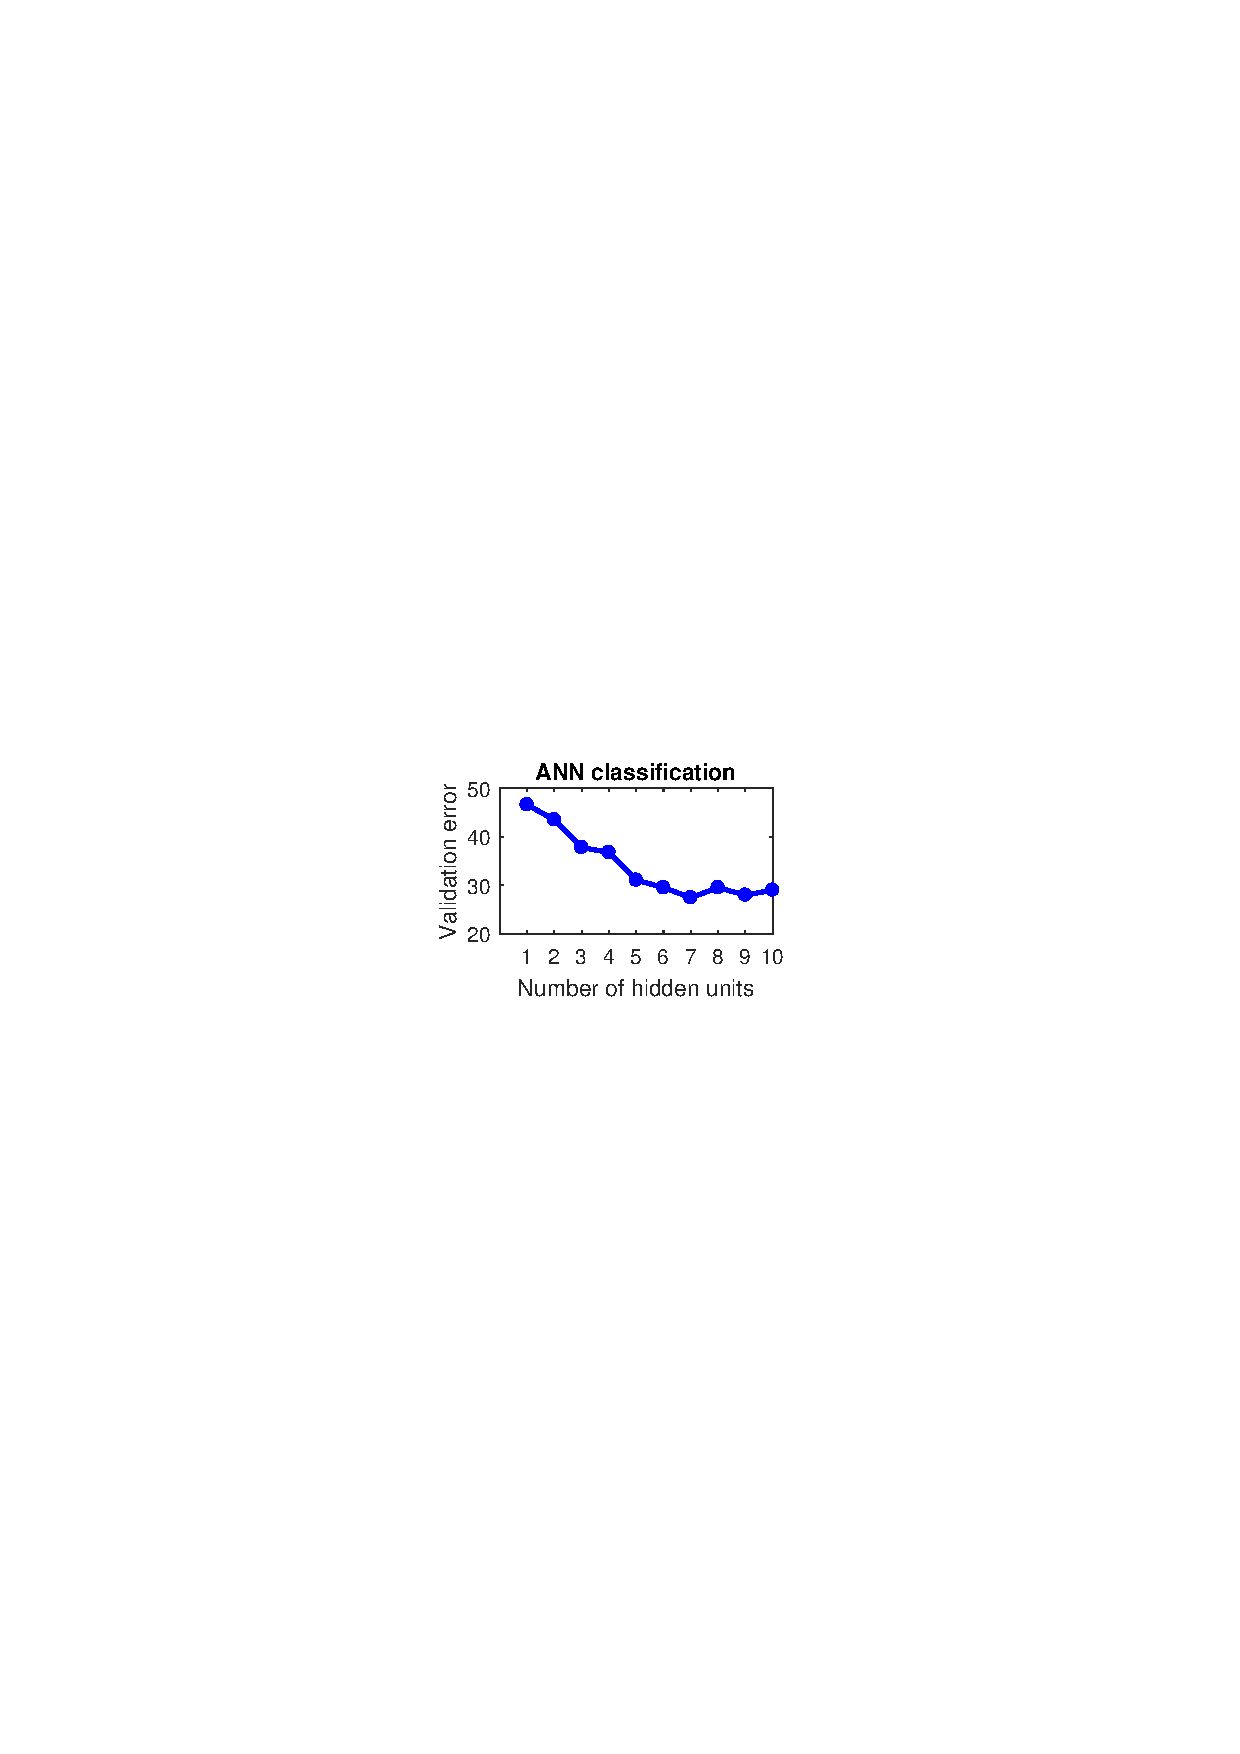
\includegraphics[width=0.40\textwidth]{fig/classification/ANN_class_validation_error.pdf}
    \caption{Validation error as a function of number of hidden units $H$. The algorithm chose $H=7$.}
    \label{fig:ANN_class_validation_error}
\end{figure}


\begin{figure}[H]
\centering
    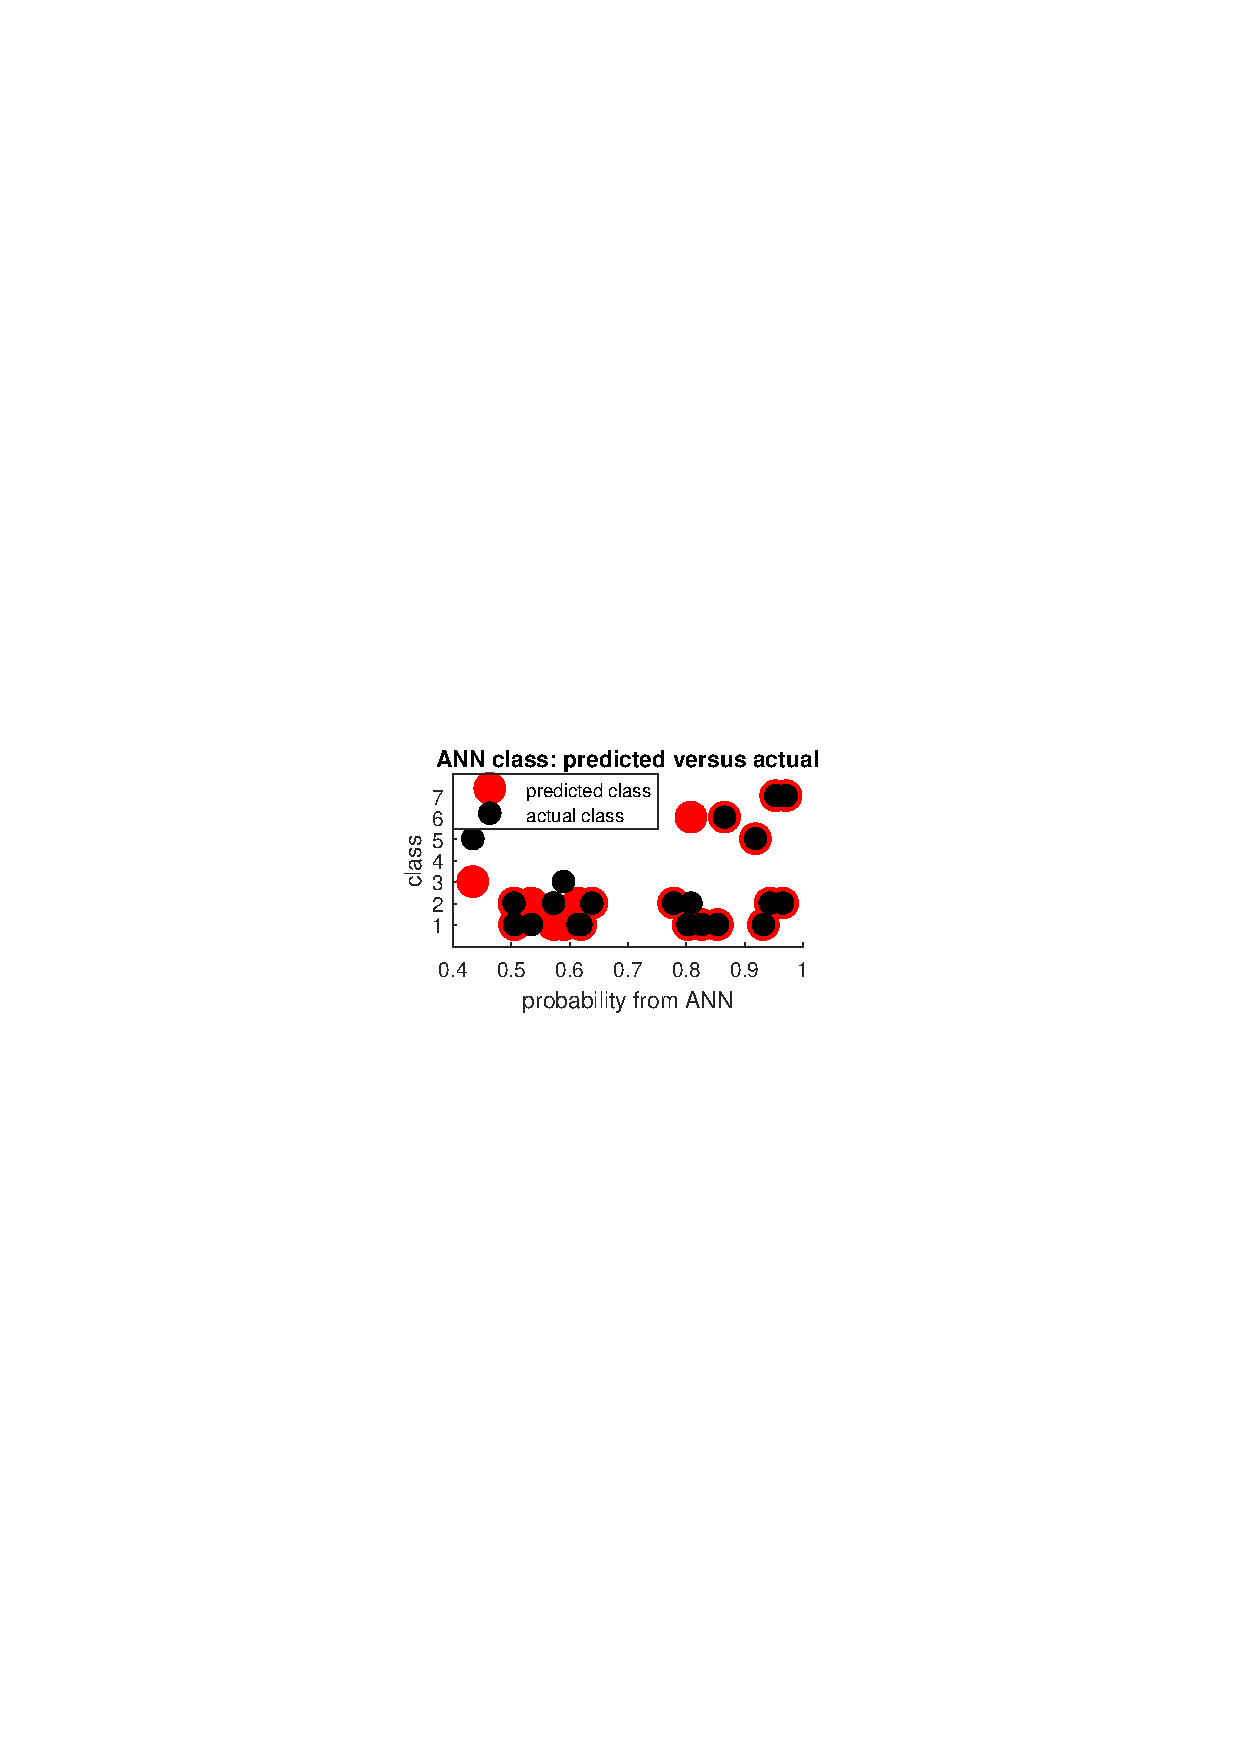
\includegraphics[width=0.45\textwidth]{fig/classification/ANN_class_predicted_vs_actual.pdf}
    \caption{Predicted class versus actual class in the final test of the ANN model with $H=7$.}
    \label{fig:ANN_class_predicted_vs_actual}
\end{figure}
\end{multicols}

